\documentclass{article}
\usepackage{pdfpages}
\usepackage{listings}
\usepackage[T1]{fontenc}
\usepackage{xcolor}
\usepackage{placeins}
\usepackage{float}
\usepackage{underscore}
\usepackage[bookmarks=true]{hyperref}
\usepackage[utf8]{inputenc}
\usepackage[margin=0.5in]{geometry}
\usepackage{graphicx}
\usepackage{subfigure}
\usepackage[english]{babel}
\hypersetup{
	bookmarks=false,    % show bookmarks bar?
%	pdftitle={Text Analytics Tutorial 4},    % title
	pdfauthor={Adam-Ryan},                     % author
	pdfsubject={TeX and LaTeX},                        % subject of the document
	pdfkeywords={TeX, LaTeX, graphics, images}, % list of keywords
	colorlinks=true,       % false: boxed links; true: colored links
	linkcolor=blue,       % color of internal links
	citecolor=black,       % color of links to bibliography
	filecolor=black,        % color of file links
	urlcolor=blue,        % color of external links
	linktoc=page            % only page is linked
}%
\def\myversion{1 }
\date{}
%\title
\usepackage{hyperref}
\begin{document}
	
\section{Exercise 1}
This is the answer to question 1.
\begin{enumerate}
	
	\item I chose the topic 'Climate change' and pulled text snippets from Twitter as I observed that commentators repeatedly use comments with a nationalistic or multi-generational focus when discussing the topic. I have removed stop words using nltk.corpus.stopwords.words, and I have normalised the words similar to my assignment one submission by lowercasing the text, removing contractions, replacing digits with numbers, and stripping punctuation. The resultant tweets are:
		\begin{verbatim}
			1 = ['anyone', 'say', 'patriotic', 'love', 'country', 'refuse', 'act', 'drought', 'flooding', 'forest'
			, 'fires', 'extreme', 'weather', 'disturbances', 'cause', 'nation', 'much', 'destruction', 'climate'
			, 'change', 'real', 'us', 'must', 'lead', 'way', 'combating']
			2 = ['global', 'south', 'suffering', 'gap', 'climate', 'change', 'research', 'rich', 'countries', 'drive'
			, 'agenda', 'studies', 'suggest', 'cbc', 'news']
			3 = ['moderate', 'vs', 'progressive', 'thing', 'survival', 'vs', 'complete', 'utter', 'catastrophe', 
			'thing', 'reconciliation', 'might', 'last', 'best', 'chance', 'fight', 'climate', 'change'
			, 'transformative', 'investments', 'next', 'generation', 'looks', 'us', 'let']
			4 = ['could', 'afford', 'give', 'wealthiest', 'americans', 'tax', 'break', 'trump', 'afford', 'stop'
			, 'climate', 'change', 'build', 'physical', 'human', 'infrastructure', 'next', 'century', 'right']
			5 = ['climate', 'crisis', 'driving', 'severe', 'drought', 'across', 'american', 'west', 'wildfires'
			, 'water', 'shortages', 'communities', 'feeling', 'impact']
			6 = ['last', 'time', 'wv', 'csn', 'tour', 'warned', 'drink', 'water', 'hotel', 'due', 'recent', 'toxic'
			, 'spill', 'forgot', 'took', 'sip', 'ended', 'urgent', 'care', 'sure', 'leave', 'climate', 'change'
			, 'funding', 'bill', 'please', 'energy', 'committee', 'chair', 'joe', 'manchin']
			7 = ['sad', 'human', 'species', 'going', 'destroy', 'climate', 'change', 'amount', 'people'
			, 'hoard', 'obscene', 'amount', 'money', 'money', 'thing', 'made', 'value', 'say', 'clearly'
			, 'value', 'lives', 'survival']
			8 = ['fifty-one', 'senators', 'oppose', 'legislation', 'stem', 'tide', 'climate', 'change'
			, 'inaction', 'profoundly', 'effect', 'quality', 'life', 'health', 'entire'
			, 'ecosystem', 'children', 'children', 'clearly', 'care', 'enough', 'future', 'generations', 'get', 'past', 'partisan', 'views']
			9 = ['climate', 'change', 'given', 'attention', 'deserves', 'politicians', 'stripes', 'would', 'working'
			, 'towards', 'solutions', 'enormously', 'frustrating', 'protecting', 'future', 'planet', 'often'
			, 'treated', 'controversial', 'political', 'issue']
			10 = ['compare', 'contrast', 'one', 'leader', 'spent', 'day', 'painting', 'lavish', 'marbella', 'villa', 
			'country', 'suffers', 'crisis', 'representing', 'scotland', 'world', 'stage', 'fostering', 'relations'
			, 'countries', 'help', 'combat', 'climate', 'change']
		\end{verbatim}
	\item 
		\begin{itemize}
	\item The word cloud with minimum frequency of one is seen in figure \ref{q1p2} which shows how a few words are repeated in the sets of tweets.:
		\begin{figure}[!h]
		\centering
		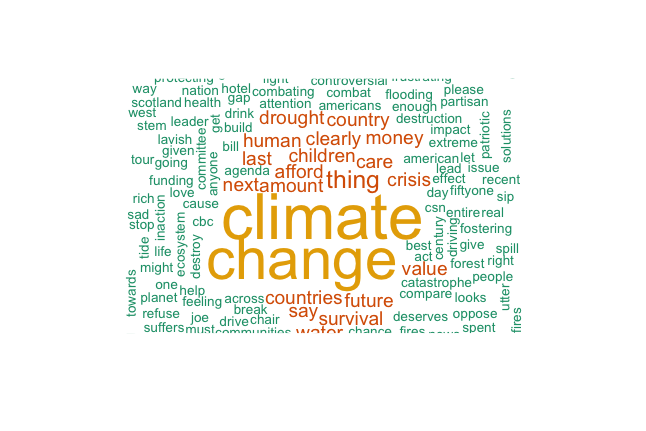
\includegraphics[width=0.6\linewidth]{climate_change_tweets.png}
		\caption{Question 1 Part 2 Word Cloud}\label{q1p2}
	\end{figure}
	\item A sample of the TF, using the count of the word across both all documents and each individual document (this was done as the text is ambiguous as to whether to consider it within the one document or across all ten) is below in figure \ref{tf} which captures the count of occurrences of words in the text after all stopwords are removed.
			\begin{figure}[!h]
		\centering
		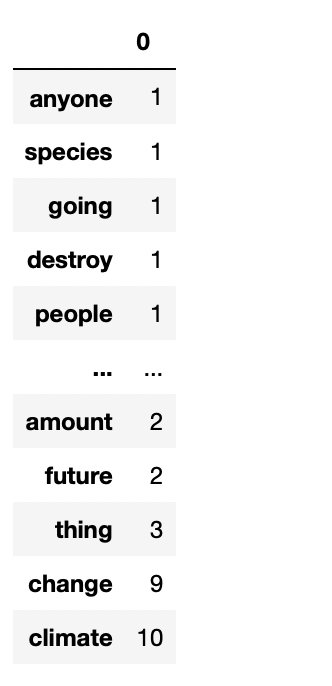
\includegraphics[width=0.2\linewidth]{tf.png}
		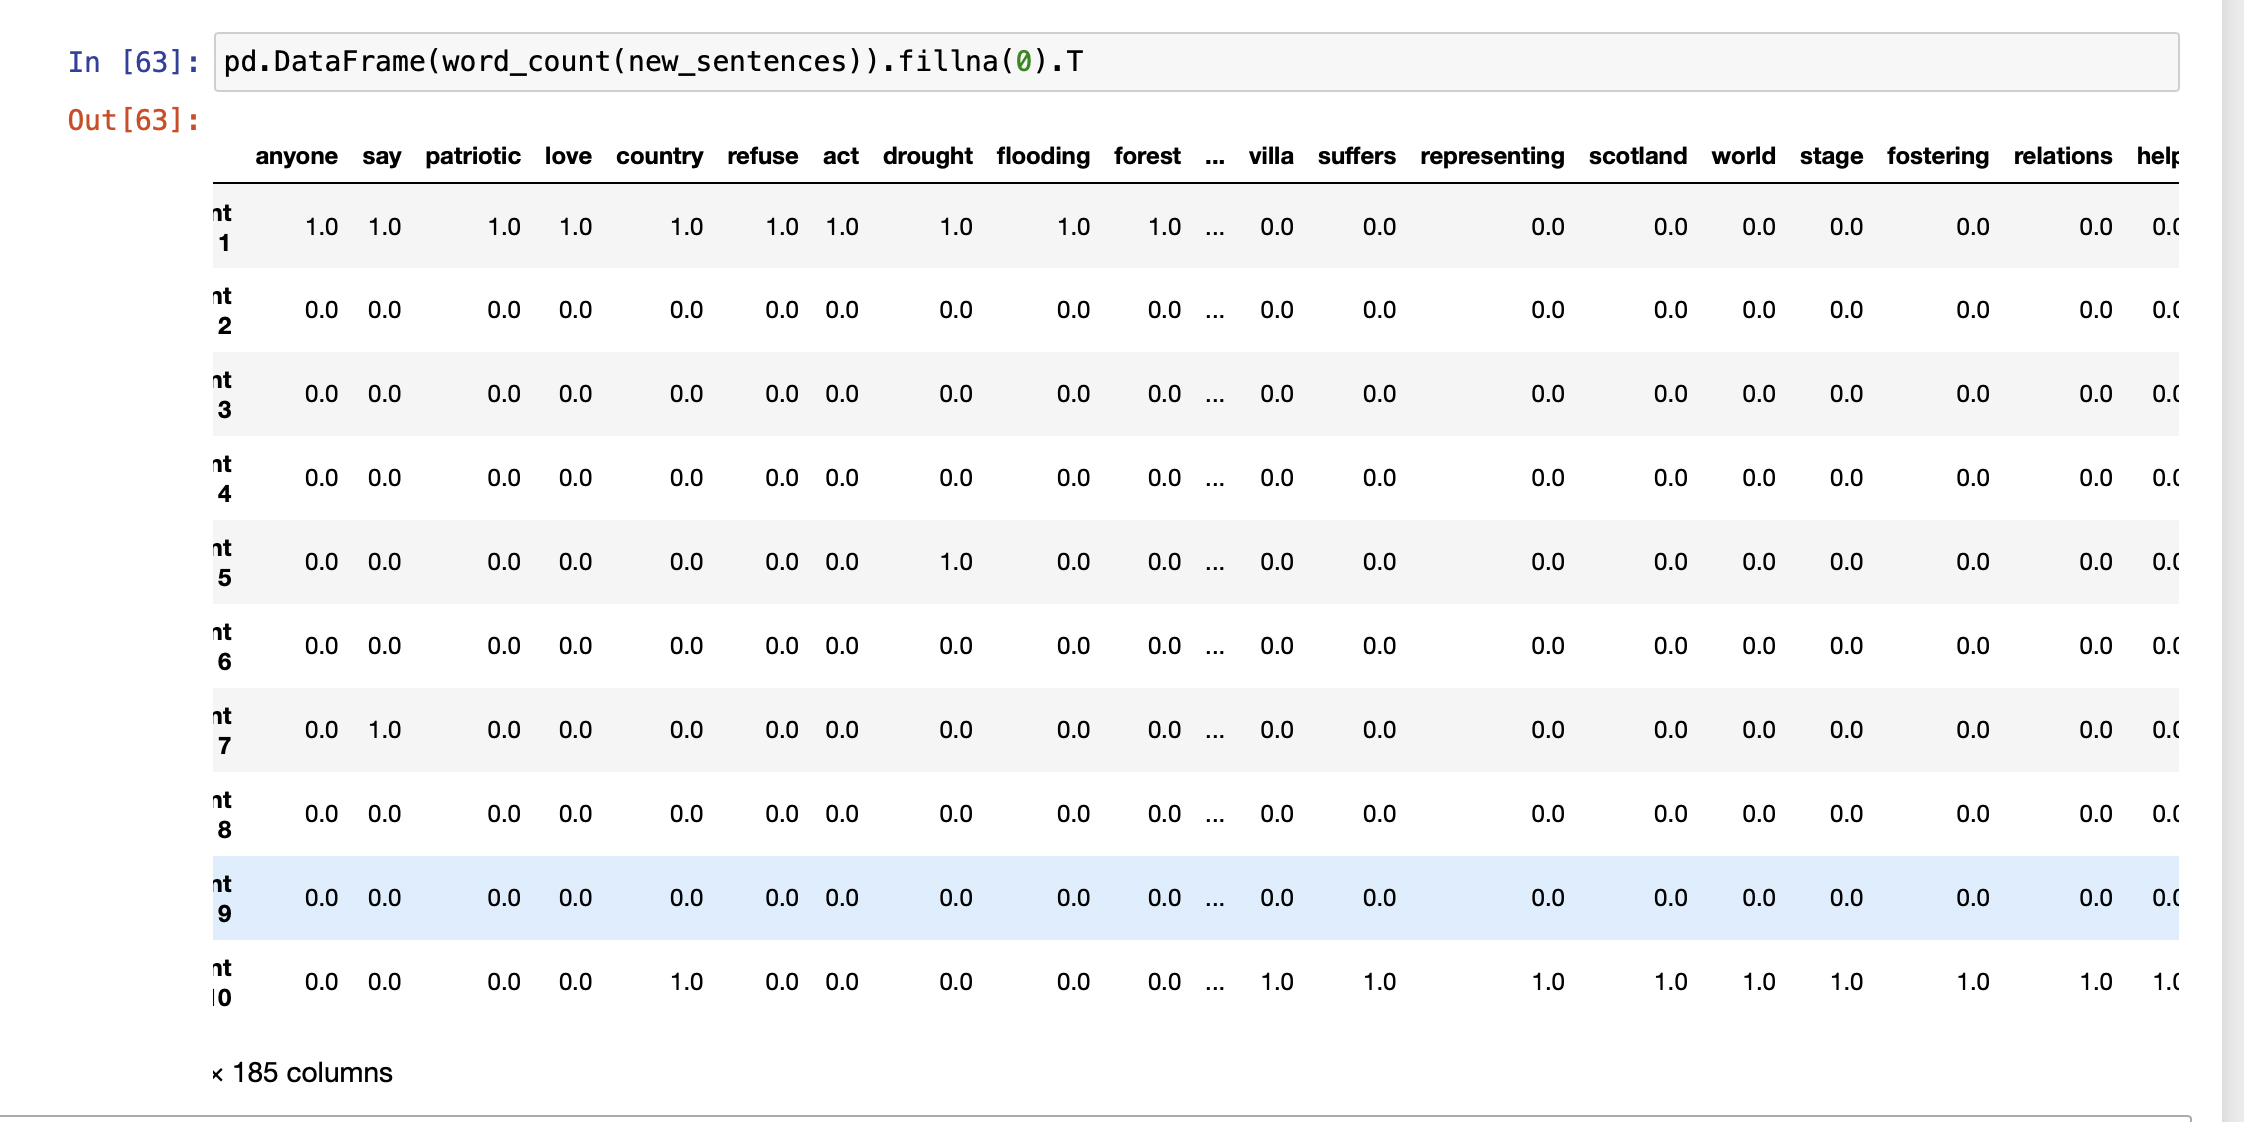
\includegraphics[width=0.4\linewidth]{tf_per_doc.png}
		\caption{Question 1 Part 2 TF}\label{tf}
	\end{figure}
	
	\end{itemize}
	\item 
	\begin{itemize}
		\item The TF-IDF is:
		\begin{figure}[!h]
			\centering
		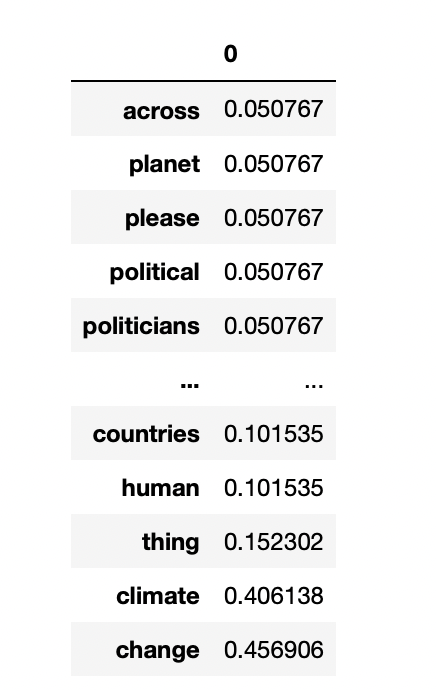
\includegraphics[width=0.2\linewidth]{tfidf_all.png}\
		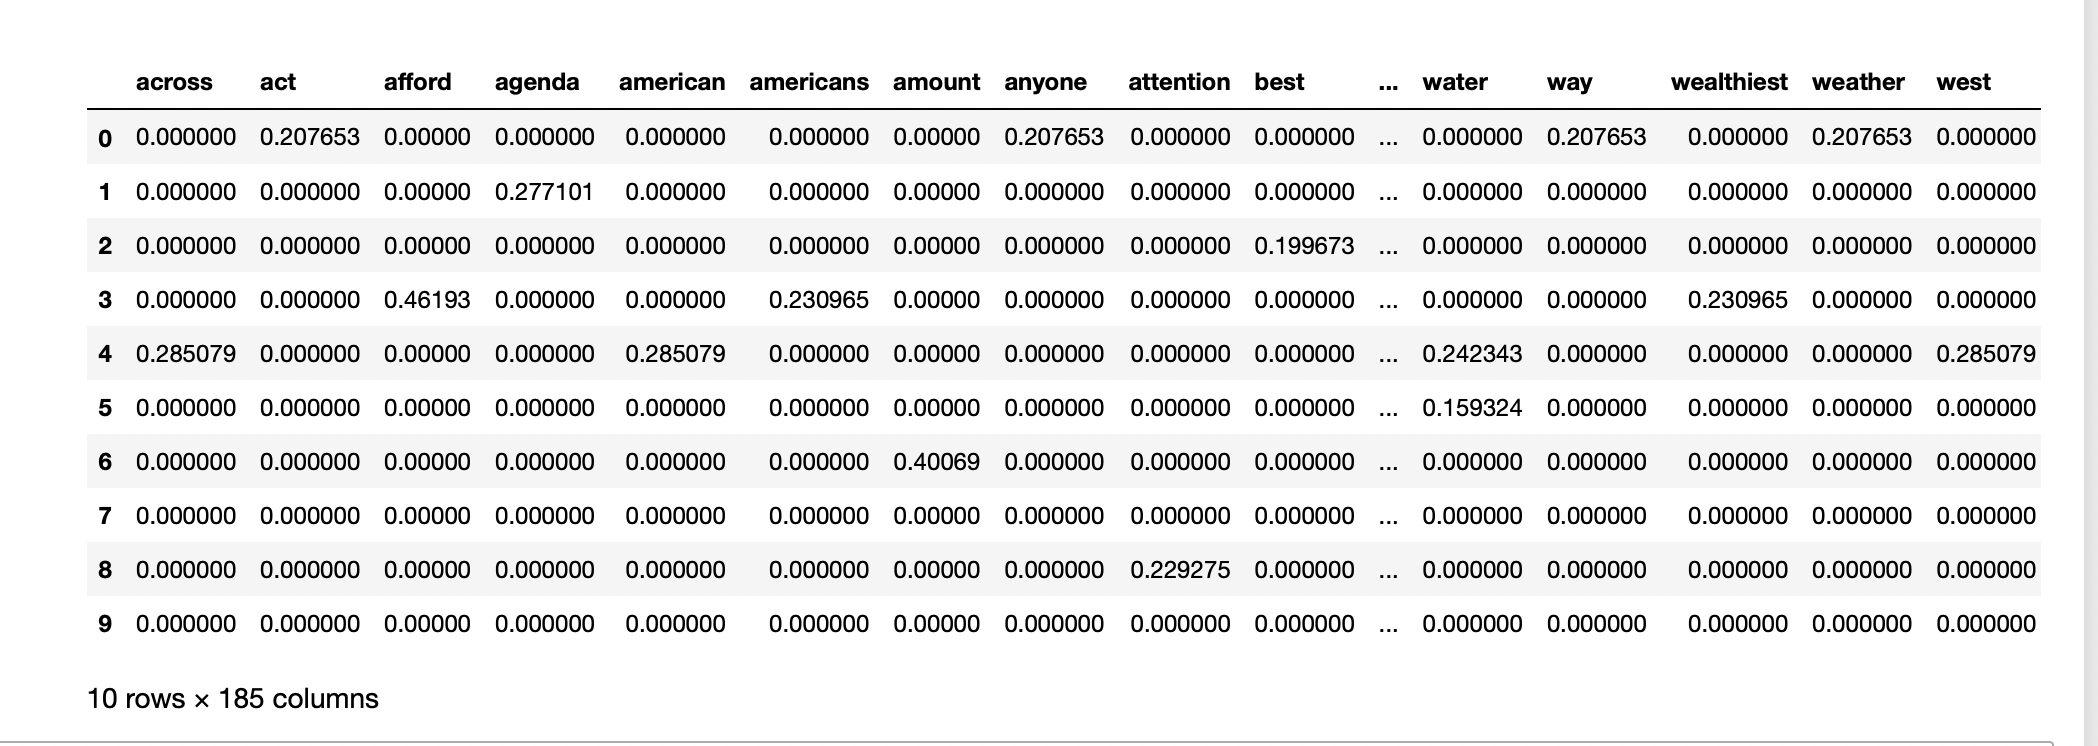
\includegraphics[width=0.6\linewidth]{tfidf.png}
		\caption{Question 1 Part 3}\label{tfidf}
	\end{figure}
	\end{itemize}

	\item In terms of the rankings there is minimal changes in the ranking between TF and TF-IDF. For the tweets I have chosen, I believe this is largely driven by the fact that although these tweets share some words and common sentements, the overall overlap between the words and tweets is relatively low. Outside of climate and change, the majority of words appear one or two times which results in a low difference between the two for the overall ranking for the documents I've chosen.
\end{enumerate}

	

\section{Exercise 2}

\begin{enumerate}
	\item I compute the top ten PMI scores by using nltk.collocations. The top ten PMI scores are:
	\begin{verbatim}
{('day', 'painting'): 7.813781191217037,
	('painting', 'lavish'): 7.813781191217037,
	('lavish', 'marbella'): 7.813781191217037,
	('marbella', 'villa'): 7.813781191217037,
	('representing', 'scotland'): 7.813781191217037,
	('scotland', 'world'): 7.813781191217037,
	('world', 'stage'): 7.813781191217037,
	('stage', 'fostering'): 7.813781191217037,
	('fostering', 'relations'): 7.813781191217037,
	('help', 'combat'): 7.813781191217037}
	\end{verbatim}
\item The results do not make sense in our example. We see that most of the bigrams which are present occur very infrequently (most occurrences in fact only occur a single time); for example help and combat have a PMI of 7.8 when, in our set, we would anticipate climate and change to have the highest PMI in our example. Applying a filter on the number of occurences as 2 minimum, we see in fact that we are left with a single result which confirms that our PMI results above are biased by single occurence bigrams:
\begin{verbatim}
	{('climate', 'change') : 4.491853096329675}
\end{verbatim}

\end{enumerate}

\section{Exercise 3}

\begin{enumerate}
	\item
	\begin{itemize}
	 \item spam\_set=['Buy MAC StudioFlix best price click here free cheap good quality free shipping'
	,'Best price on MAC StudioFlix purchase now before time runs out go now limited time only for cheap prices and free delivery'
	,'Shop StudioFlix today and avail of great prices low low costs and cheap shipping only available today'
	,'Visit here and buy StudioFlix before time runs out on our great offers and low costs before sale ends tomorrow'
	,'Sale ending soon shop StudioFlix today before your chance to purchase with free delivery runs out now! Buy today!'
	,'Shop StudioFlix now for amazing lashes only at our website. Lowest price low cost with free shipping.'
	,'Cheap studioFlix available here today click now low prices with free shipping and good service'
	,'Great offer on StudioFlix only at our website click here for best price now and fantastic deals'
	,'Buy StudioFlix today for vibrant lashes and fantastic makeup available on discount for a limited time only buy now before you miss your chance'
	,'StudioFlix discount ending soon. Youre about to lose your chance of an amazing discount with speedy next day delivery free only here']
	\item random\_set=[
	"""
	When teaching him a few years back, there was a palpable sense that students were connecting with his work. We wrote letters to him, he then called to say thank you for taking the time to write. He was genuinely touched. He sent a signed copy of a poem too. A gent. RIP
	"""
	,"""
	68 percent of small businesses surveyed in the EU who use personalised advertising said it is an effective way to find new customers. Just like Mami Poppins.
	"""
	,"""
	FAI to put faith in Stephen Kenny with new contract as Ireland manager
	"""
	,"""
	In Trinity we had such good fun together. He loved walking around Dublin at dawn. R.I.P. Brendan Kennelly recites Begin at Listowel Writers' Week 
	"""
	,"""
	If you missed the one-off in-cinema screening of DWELLING IN THE FUCHUN MOUNTAINS as part of 
	@EastAsiaFFIrl
	Discoveries, great news - it is now available to watch online! 
	"""
	,"""
	Join dynamic alumni Nicai de Guzman (Wolfgang Digital), Emmet Daniel (Hubspot), and expert Dr. Linda Yang (Intercultural Development Programme, UCD) as they offer advice on thriving in multicultural work environments
	"""
	,"""
	Deceit, treason and rivalry returns with \#Succession S3. Starts 18 October, exclusively on Sky.
	"""
	,"""
	It’s 2021. You don’t have to put corporate lobbyists over people to legislate, fundraise, and win. 
	
	It’s insulting to tell everyday people who worked tirelessly for a majority that they must suffer insane drug prices,no voting rights,\& climate disaster for political convenience.
	"""
	,"""
	Maths Week will take place from October 18th-22nd. Activities in class will include Maths Minutes, Einstein's Riddle and Maths Dingbats. Keep an eye on Twitter for daily puzzles
	"""
	,"""
	Metal gear solid 4 fan art (no criticism allowed)
	"""
	,"""
	This page is a timeline of Tweets with information and advice from the Taoiseach and Tánaiste, the Minister for Health and other ministers, the Department of Health, the HSE and public health authorities across the Republic of Ireland. For more, visit: 
	"""]
	\end{itemize}
\item NLTK has an entropy formula located \href{https://www.nltk.org/book/ch06.html}{here} which is what was used to generate the entropy. 
\begin{verbatim}
	import math
		def entropy(labels):
		freqdist = nltk.FreqDist(labels)
		probs = [freqdist.freq(l) for l in freqdist]
		return -sum(p * math.log(p,2) for p in probs)
\end{verbatim}
	We see the following entropy is generated over the spam set, random set, and the spam and random sets combined
		\begin{figure}[!h]
	\centering
	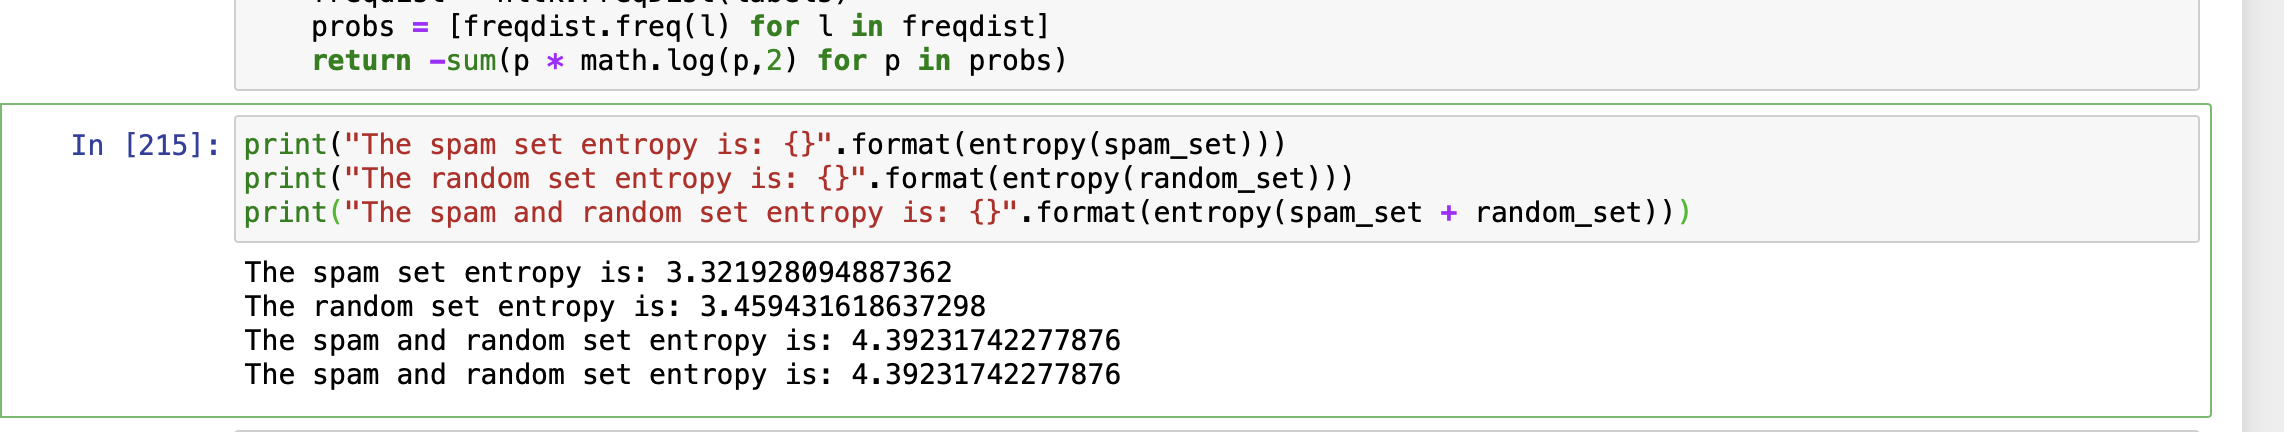
\includegraphics[width=0.75\linewidth]{entropy.png}
	\caption{Entropy}\label{ent}
\end{figure}
In what we generated, unsurprisingly the spam set, which is similar in its promotion of Mac StudioFlix in a sale context, has a lower entropy than a set of tweets which were chosen at random from my timeline. Unsurprisingly, combining the fake spam tweets and the random tweets has the highest entropy.
\end{enumerate}


\end{document}
